\chapter{Wobbling Motion in Nuclei}

The pioneering work of Bohr and Mottelson \cite{bohr1998nuclear} which was done more than 50 years ago lead to some interesting features regarding the collective phenomena in triaxial nuclei. Namely, they pointed out that a specific precessional motion of the nucleus's spin will take place when the rotational energy is sufficient. The angular momentum for triaxial nuclei is not aligned any of the principal axes of the ellipsoid, but it \emph{precesses} and \emph{wobbles} around one of these axes. They called this phenomenon \textbf{wobbling motion} (w.m.).
This combined motion comes from a consequence regarding the MOI. Indeed, the asymmetry of the three MOI makes the quantum mechanical nature of rotation to be possible around any of the three axes. As such, a \emph{main} rotation around the axis with the largest MOI will be the most energetically favorable, but the other two directions can \emph{quantum mechanically disturb} this main rotation, leading to this unique characteristic of triaxial nuclei.

The non-uniformity nature of w.m. was firstly studied for the `pure' rigid-rotators that correspond to the even-even nuclei. In this case, the w.m. can be treated as small amplitude oscillations of the total angular momentum $\mathbf{I}$ around the axis corresponding to the largest MOI.

\section{Wobbling Motion in Even-Even Nuclei}

The analytical expressions for wobbling excitations were firstly evaluated by Bohr and Mottelson using the so-called \emph{Harmonic Approximation} (HA). This can be described as a small-amplitude limit for the Triaxial Rigid Rotor Hamiltonian that was discussed in Chapter \ref{chapter4} (see Section \ref{trm-model}). In this limit, the projection of the total angular momentum onto the axis with largest MOI can be approximated $I_3\approx I$, meaning that the nucleus will do most of its rotation around this axis, with some `disturbance' from the other two principal of the triaxial rotor. 

For the description of this simple wobbler, one can consider the case when the $3$-axis has the largest MOI, and the following order holds true:
\begin{align}
    \mathcal{I}_3>\mathcal{I}_2>\mathcal{I}_1\ ,
\end{align}
or equivalently:
\begin{align}
    A_3<A_2<A_1\ .
\end{align}
The Hamiltonian can be written as:
\begin{align}
    \hat{H}_\text{rot}={\color{red}A_3I_3^2}+{\color{blue}\left(A_1I_1^2+A_2I_2^2\right)}
    \label{general-rotor-ham-evenA}
\end{align}

The different colors from Eq. \ref{general-rotor-ham-evenA} try to emphasize the fact that a Hamiltonian for the simple wobbler can be regarded as \emph{a main rotation around $3$-axis} (represented by red color) and \emph{the (precession + oscillation) of the total angular momentum} (represented by blue color).

The wobbling excitations which cause oscillations with small amplitudes for $\mathbf{I}$ about the $3$-axis are assumed to have a harmonic-like behavior, meaning that the final energy spectrum of a simple wobbler (even-even nucleus) will have the typical $\hbar\omega(n+1/2)$ behavior. Since this oscillator motion can be explained as `vibrations' of the total angular momentum around a steady position, where each wobbling excitation consists of an additional vibrating phonon, one can express the Hamiltonian in terms of \emph{boson} creation and annihilation operators. As such, the quantum mechanical treatment implies \cite{bohr1998nuclear}:
\begin{align}
    b^\dagger=\frac{1}{\sqrt{2I}}I_+\ ,\ b=\frac{1}{\sqrt{2I}}I_-\ ,\ \left[b,b^\dagger\right]\approx 1\ .
\end{align}

This initial quantization allows one to write Eq. \ref{general-rotor-ham-evenA} as a rotational term and a wobbling-specific one:
\begin{align}
    \hat{H}_\text{rot}&={\color{red}A_3I_3^2}+{\color{blue}H_w}\ ,\label{rot-ham-non-diagonal} \\
    {\color{blue}H_w}&={\color{blue}t_1\left(n+\frac{1}{2}\right)+\frac{1}{2}t_2(b^\dagger b^\dagger + bb)}\ ,
    \label{wob-ham-non-diagonal}
\end{align}
where the \emph{number of boson excitations} is denoted by $n$ and it is given by $n=b^\dagger b$. Each wobbling quanta will carry an angular momentum of one unit less with respect to the $3$-axis. The two factors $t_{1,2}$ are expressed in terms of the inertial parameters as \cite{bohr1998nuclear}:
\begin{align}
    t_1&=I(A_2+A_1-2A_3)\ , \\
    t_2&=I(A_2-A_1)\ .
\end{align}

Notice the linear dependence of the two parameters on the total angular momentum $I$. Moreover, depending on the values of $A_k$, the contribution of $t_{1,2}$ can be negative. Their behavior is shown within the right inset of Fig. \ref{fig-even-even-wobbling-energies}. Although the Hamiltonian $H_w$ is considered to have an oscillator-like behavior, its general expression does not look like a typical harmonic Hamiltonian. For this, the Hamiltonian given in Eq. \ref{wob-ham-non-diagonal} can be brought to a diagonalized form by introducing a new set of boson creation and annihilation operators. These operators will be written as linear combinations of $(b^\dagger,b)$:
\begin{align}
    c^\dagger=w_1b^\dagger-w_2b\ ,\\
    c=w_1b-w_2b^\dagger\ ,
\end{align}
where the two coefficients $w_{1,2}$ are defined in terms of $t_{1,2}$ as:
\begin{align}
    w_1&=\left[\frac{1}{2}\left(\frac{t_1}{\sqrt{t_1^2-t_2^2}}+1\right)\right]^{1/2}\ ,\nonumber\\
    w_2&=\left[\frac{1}{2}\left(\frac{t_1}{\sqrt{t_1^2-t_2^2}}-1\right)\right]^{1/2}\ .
    \label{eqs-w1-w2-terms-wobbling}
\end{align}

The terms $w_{1,2}$ verify the condition $w_1^2-w_2^2=1$ and they make the `dangerous' products ($b^\dagger b^\dagger$,$bb$) disappear in this new representation \cite{oi2006semi}. Note that there is no spin dependence inferred in Eq. \ref{eqs-w1-w2-terms-wobbling} such that $w_{1,2}$ are constant functions of spin, unlike the coefficients $t_{1,2}$. Moreover, introducing a number operator $\hat{n}=c^\dagger c$ and the excitation quanta $\hbar\omega_w$ defined as:
\begin{align}
    \hbar\omega_w=\sqrt{t_1^2-t_2^2}=2I\sqrt{(A_1-A_3)(A_2-A_3)}\ ,
    \label{wobbling-frequency-even-A}
\end{align}
then a final expression of $H_w$ can be expressed, which has a behavior typical to the \emph{harmonic oscillator}:
\begin{align}
    H_w=\hbar\omega_w\left(\hat{n}+\frac{1}{2}\right)\ .
    \label{wob-ham-diagonal}
\end{align}

In this expression, the excitation quanta $\hbar\omega_w$ which was defined in Eq. \ref{wobbling-frequency-even-A} in terms of $t_{1,2}$ is called \emph{wobbling frequency} and its increasing linearly with the total angular momentum. Accordingly, Eq. \ref{rot-ham-non-diagonal} can be re-written with the wobbling Hamiltonian defined in Eq. \ref{wob-ham-diagonal}:
\begin{align}
    \hat{H}_\text{rot}=A_3I(I+1)+\hbar\omega_w\left(\hat{n}+\frac{1}{2}\right)\ .
    \label{rot-wob-ham-diagonal}
\end{align}

Thus, in the HA, the eigenvalues of the rotor Hamiltonian can be expressed in terms of a \emph{wobbling phonon number} $n_w$ (which is the eigenvalue of the number operator $\hat{n}=c^\dagger c$) and a \emph{wobbling frequency} (defined in Eq. \ref{wobbling-frequency-even-A}):
\begin{align}
    E_{I,n}={\color{red}A_3I(I+1)}+{\color{blue}\hbar\omega_w\left(n_w+\frac{1}{2}\right)}\ .
    \label{eq-wobbling-energy-evenA}
\end{align}

The spectrum for an even-even wobbling nucleus is thus represented by Eq. \ref{eq-wobbling-energy-evenA}. Notice again the two colored terms that illustrate the energy coming from the rotation around the $3$-axis and the disturbed motion with small oscillations around the other two axes. Consequently, the wobbling character of the system will be generated by the latter harmonic term. The wobbling phonon number $n_w$ is related to the `strength' of the tilting for $\mathbf{I}$, indicating the fact that an increasing number for $n_w$ will result in oscillations with larger amplitudes around the other two axes. The phonon number takes values $n_w=0,1,\dots$. In inset $b)$ from Fig. \ref{wobbling-geometry-tilting-sketch}, a sketch which shows the tilting effect that the wobbling phonon number has on the total angular momentum vector is drawn. For completeness, the collective structure of two wobbling bands generated through phonon excitations is exemplified in inset $a)$ from Fig. \ref{wobbling-geometry-tilting-sketch}.

\begin{figure}
    \centering
    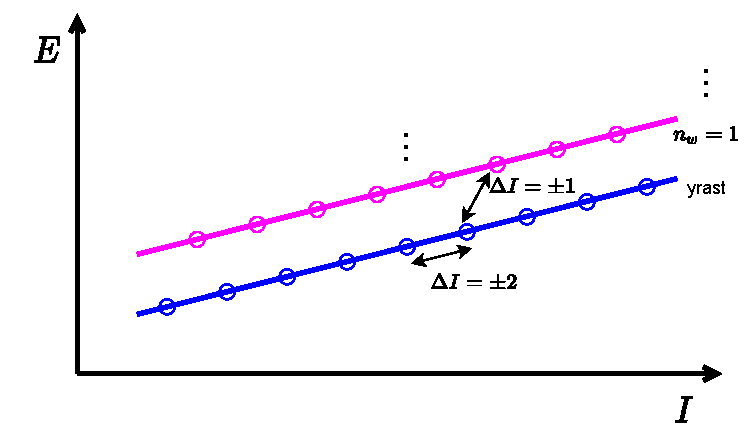
\includegraphics[scale=0.72]{Chapters/Figures/wobbling_n_schematic-1.pdf}
    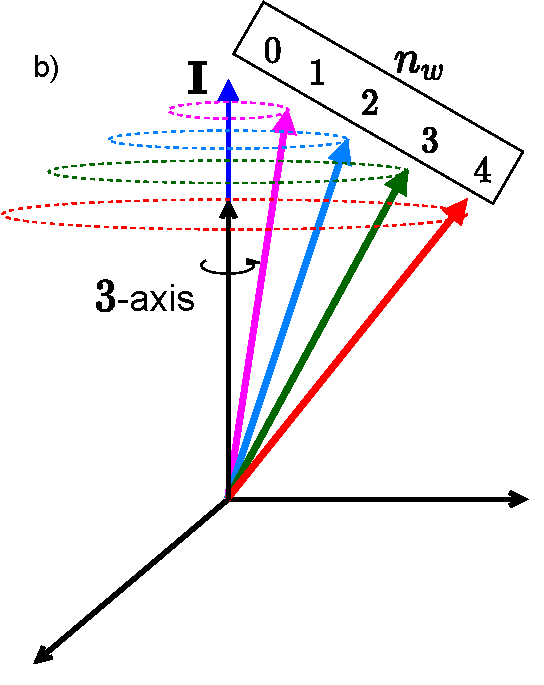
\includegraphics[scale=0.6]{Chapters/Figures/wobbling_n_schematic-2.pdf}
    \caption{\textbf{Left:} A typical wobbling structure for even-even nuclei. The yrast band contains even values of spins since the band has signature $\alpha=0$, while the first excited band has odd spins and $\alpha=1$. The intraband states differ by 2 units of angular momenta, while the interband ones differ with only one unit. \textbf{Right:} The increase of tilting angle between the rotational axis (the $3$-axis in this case) and the total angular momentum $\mathbf{I}$. With each wobbling phonon number, the total angular momentum tilts more and more, generating a `stronger' precessional motion (illustrated by the colored ellipses).}
    \label{wobbling-geometry-tilting-sketch}    
\end{figure}

An alternative way of depicting the wobbling term $H_w$ from Eq. \ref{rot-ham-non-diagonal} would be to express it more generally, in terms of $I_2$ and $I_3$. When doing so, one achieves the following form (assuming that rotation is around the $3$-axis) \cite{oi2006semi}:
\begin{align}
    % H_w={\color{magenta}(A_1-A_3)I_1^2}+{\color{orange}(A_2-A_3)I_2^2}={\color{magenta}T_\text{kin}}+{\color{orange}T_\text{pot}}\ ,
    H_w=(A_1-A_3)I_1^2+(A_2-A_3)I_2^2=T_\text{kin}+T_\text{pot}\ ,
\end{align}
where according to Ref. \cite{wen2015wobbling}, one can regard these two factors as a \emph{kinetic} and a \emph{potential} term. This way of expressing $H_w$ is instructive since it keeps a close contact with the `classical' picture of understanding the total energy of a system.

As a quantitative analysis of the wobbling frequency and the rotor energy, one can take three arbitrary values for the moments of inertia (and, implicitly, the inertia factors $A_k$) and see the behavior of both $E_{I,n}$ and $\hbar\omega_w$ with increasing angular momentum and wobbling phonon number. Keep in mind that depending on the value of the wobbling phonon number, different spin sequences will be allowed. More precisely, from the invariance of the rotor w.r.t. rotations by $\pi$ about the principal axes for even-even nuclei, the signature quantum number $\alpha$ can take the values 0 and 1. Each wobbling band will have an alternating signature, starting with $\alpha=0$ for $n_w=0$ then $\alpha=1$ for $n_w=1$ and so on: even spin sequences appear for even values of $n_w$ and odd spin sequences appear for odd values of $n_w$ (see Fig. \ref{fig-even-even-wobbling-energies}).

The rotor energy from Eq. \ref{eq-wobbling-energy-evenA} is graphically represented for an arbitrary set of moments of inertia as a function of the nuclear angular momentum $I$ in Fig. \ref{fig-even-even-wobbling-energies}. This pedagogical example contains rotational bands up to $n_w=5$ in the wobbling phonon number. From Fig. \ref{fig-even-even-wobbling-energies}, one can see the linear dependence on the total angular momentum and, moreover, the wobbling energy and frequency both are increasing with spin.

\begin{figure}
    \centering
    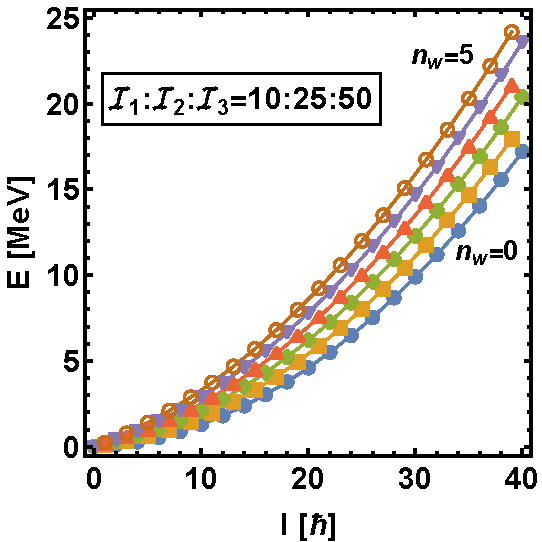
\includegraphics[scale=0.7]{Chapters/Figures/wobbling-evenA.pdf}
    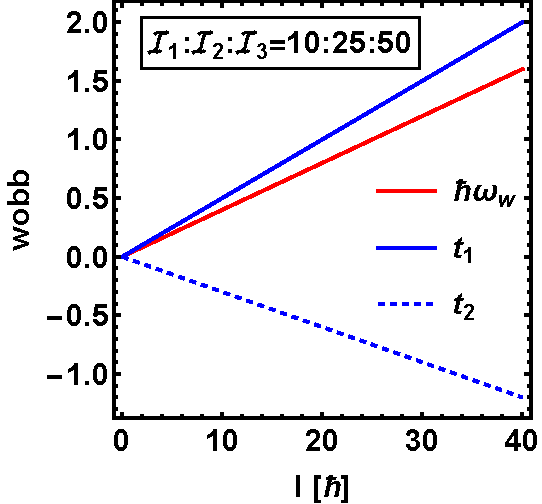
\includegraphics[scale=0.74]{Chapters/Figures/wobblingFreq-evenA.pdf}
    \caption{\textbf{Left:} The energy spectrum for an even-even nucleus with three different moments of inertia, with the main rotation around the $3$-axis, according to Eq. \ref{eq-wobbling-energy-evenA}. Each wobbling band has alternating signature number $\alpha$ (starting with $\alpha=0$ for the ground state $n_w=0$ band). Notice the even/odd spin sequences for each band. \textbf{Right:}: The wobbling frequency plotted together with the linear terms $t_1$ and $t_2$ that are used to express $\hbar\omega_w$. Same set of MOI were used across both figures and the unit for $\mathcal{I}_i$ is $\hbar^2\ \text{MeV}^{-1}$.}
    \label{fig-even-even-wobbling-energies}
\end{figure}


Another instructive analysis would be the evolution of the components of $\mathbf{I}$ as functions of the polar and azimuthal angles $\theta,\varphi$. Indeed, expressing the three angular momentum components as:
\begin{align}
    I_1&=I'\sin\theta\cos\varphi\ ,\\
    I_2&=I'\sin\theta\sin\varphi\ ,\\
    I_3&=I'\cos\theta\ ,
    \label{angular-momentum-polar-components}
\end{align}
where $I'=\sqrt{I(I+1)}$, one can make a graphical representation for them, by letting $\theta$ and $\varphi$ vary within their corresponding intervals. In Fig. \ref{figs-angular-momentum-components-polar}, the quantities $I_1$ and $I_2$ are represented in the $(\theta,\varphi)$ plane for a fixed spin value $I=10\hbar$. Since the third component is independent of the azimuthal angle $\varphi$, it has been dismissed.

\begin{figure}
    \centering
    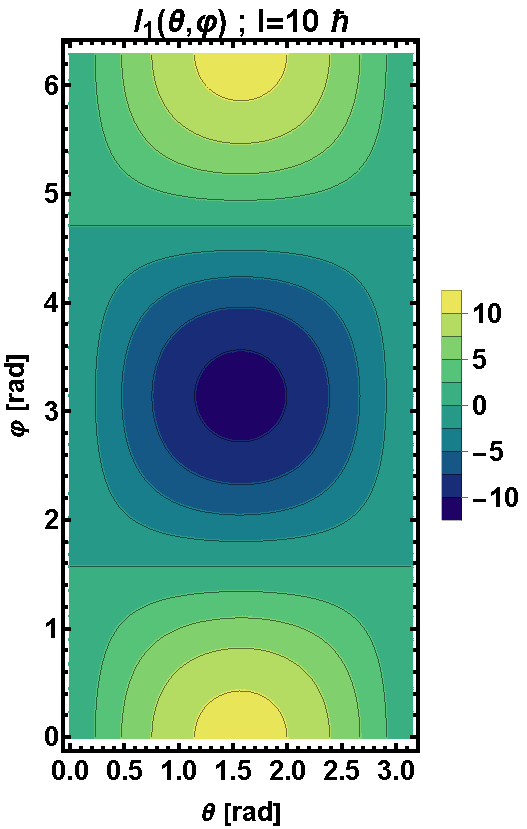
\includegraphics[scale=0.66]{Chapters/Figures/angular_components-TRM-1.pdf}
    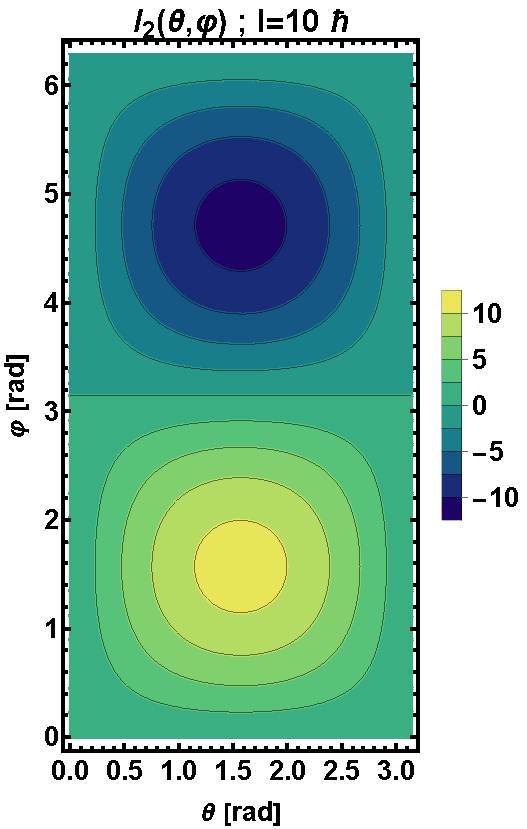
\includegraphics[scale=0.66]{Chapters/Figures/angular_components-TRM-2.pdf}
    \caption{The geometrical representation of the first and second component of the total angular momentum $\mathbf{I}$ as functions of the polar angles, according to Eq. \ref{angular-momentum-polar-components}.}
    \label{figs-angular-momentum-components-polar}
\end{figure}

The other relevant observables which can be calculated for simple wobbler within the HA are the two quadrupole moments $Q_{20,22}$ and the intraband + interband $B(E2)$ transition probabilities. The quadrupole components are expressed in terms of the intrinsic quadrupole moment $Q_0$ and the triaxiality parameter as \cite{shoji2006microscopic}:
\begin{align}
    Q_{20}=Q_0\cos\gamma\ ,\ Q_{22}=\frac{1}{\sqrt{2}}Q_0\sin\gamma\ .
    \label{quadrupole-components-q20-q22}
\end{align}

These components can be furthermore used to determine the intraband $B(E2)$ transition probabilities \cite{wen2015wobbling}:
\begin{align}
    B(E2;(n,I)\to(n,I-2))=\frac{5}{16\pi}Q_{22}^2\ ,
    \label{intraband-probability-simple-wobbler}
\end{align}
and also the interband transitions:
\begin{align}
    B(E2;(n,I)\to(n-1,I-1))&=\frac{5}{16\pi}\frac{n}{I}\left(\sqrt{3}Q_{20}w_1+\sqrt{2}Q_{22}w_2\right)^2\ , \label{interband-probability-simple-wobbler-1}\\
    B(E2;(n,I)\to(n+1,I-1))&=\frac{5}{16\pi}\frac{n+1}{I}\left(\sqrt{3}Q_{20}w_2+\sqrt{2}Q_{22}w_1\right)^2\ .
    \label{interband-probability-simple-wobbler-2}
\end{align}

Notice that for the intraband transitions, going from the state $I$ to $I-2$ will only depend quadratically on the quadrupole component $Q_{22}$, making thus the transitions spin-independent.

\subsubsection*{Triaxial rotor energy vs. wobbling energy}

An important discussion should be made regarding the nomenclature for energies when referring to wobbling motion. As shown in Eq. \ref{eq-wobbling-energy-evenA}, the energy spectrum for a simple wobbler can be determined for every phonon number and spin sequences. However, that is the `full' spectrum  of the wobbler, which is composed of the \emph{yrast} states with $n_w=0$ and the \emph{excited states} having $n_w=1,\dots$ and so on. On the other hand, the so-called \emph{wobbling energies} are defined in terms of these `absolute values' (i.e., $E_{I,n}$) with the following rules \cite{wen2015wobbling}:
\begin{align}
    E_\text{wob}(I_\text{even})&=E_{I,n}-E_{I,0}\ ,\\
    % E_\text{wob}(I_\text{even})&=E_{I,n}-E_{I,0}\ ,\nonumber \\
    E_\text{wob}(I_\text{odd})&=E_{I,n}-\frac{1}{2}\left(E_{I-1,0}+E_{I+1,0}\right)\ ,
    \label{eq-wobbling-energy-definition-evenA}
\end{align}
where the former wobbling energy corresponds to the even values of $I$ and the latter is applied for odd values of $I$. Very often within literature the energies calculated via Eq. \ref{eq-wobbling-energy-evenA} are referred to also as wobbling energies, which is not the same as Eq. \ref{eq-wobbling-energy-definition-evenA}, so a distinction should be made clear.

\subsection{Testing the Harmonic Approximation}

It is worth going further and apply the HA formalism for even-even nuclei for an existing spectrum. As such, one can take $^{130}$Ba as a testing example. As it will be discussed in a follow-up section, it turns out that experimental observations for wobbling structures in even-mass isotopes have been very scarce. Nevertheless,  very recently Petrache et al. identified a large collection of band structures in $^{130}$Ba \cite{petrache2019diversity}. Two of them are reported to be of wobbling nature \cite{chen2019transverse}. Having these two collective bands, one can check if the energy formula given in Eq. \ref{eq-wobbling-energy-evenA} for the simple wobbler can be applied for this isotope.

The method described in here will be based on a \emph{fitting procedure}, namely a set of parameters will be extracted from the expression of $E_{I,n}$ and they will adjusted such that the experimental data is best reproduced by the theoretical model. This kind of approach works really well for `well-behaved' model functions and if the input data is large enough to reach a good fit precision. More often than not, if the model function contains parameters which have a clear physical meaning then fitting becomes a suitable approach. In fact, in the following chapters, the developed formalism will verify the experimental data through similar fitting procedures (although their `core'-implementation will be more complex).

Looking at the energy formula from Eq. \ref{eq-wobbling-energy-evenA}, at a first glance, two fitting parameters would appear, namely the largest moment of inertia $\mathcal{I}_3$ and the wobbling frequency $\hbar\omega$. However, the wobbling frequency is furthermore dependent on the other two moments of inertia (as per Eq. \ref{wobbling-frequency-even-A}), meaning that one can use the set $\mathcal{P}_\text{fit}=\left[\mathcal{I}_1,\mathcal{I}_2,\mathcal{I}_3\right]$ as appropriate fitting parameters. The wobbling phonon number $n_w$ is attributed as follows: $n_w=0$ for the yrast band (denoted throughout calculations with B1) and $n_w=1$ for the first excited band (denoted with B2). The band B1 has signature $\alpha=0$ so it is the even-spin sequence, while B2 has odd spins. The experimental data regarding spins and energies for the two bands correspond to the measurements done in Ref. \cite{petrache2019diversity}.

\subsubsection*{Energy Spectrum}

Indeed, by following the procedure described above, the set $\mathcal{P}_\text{fit}$ is obtained. The parameters, i.e., the three moments of inertia are shown in Table \ref{table-params-ba130}. Remarking that fact that the largest MOI which was obtained via the fitting procedure is the one corresponding to the $3$-axis. With these parameters, the theoretical energies are determined numerically and the two bands are compared to the measured data in Fig. \ref{plot-ba130-excitation-energies}. Concerning the fitted energies, in the present calculations, instead of working with the `absolute energies' (i.e., the exact values of the energies that correspond to the measured spectrum), the \emph{excitation energies} were used instead \cite{raduta2017semiclassical,raduta2018wobbling,raduta2020towards}. These are determined by subtracting the band-head energy of B1 (the $10^+$ level) from each excited state of B1 and B2. Doing this improves the accuracy of the results. The excitation energy for a spin state $I$ is given as:
\begin{align}
    E(I)=E_\text{abs}(I)-E_\text{abs}(I_0)\ ,
    \label{excitation-energy-general-formula}
\end{align}
where `abs.' signifies the absolute value for $E$ at that particular spin state and $I_0$ is the band-head state within the yrast band.

% \begin{table}
%     \centering
%     \resizebox{0.4\textwidth}{!}{%
%     \begin{tabular}{|c|c|c|l|}
%     \hline
%     $\mathcal{I}_1$ & $\mathcal{I}_3$ & $\mathcal{I}_2$ & Unit \\ \hline
%     27 &22 &43 &$\hbar ^ 2\text{MeV} ^ {-1}$ \\ \hline
%     \end{tabular}%
%     }
%     \caption{The parameter set $\mathcal{P}_\text{fit}$ obtained from the fitting procedure of the excitation energies of the two wobbling bands (B1 and B2) for $^{130}$Ba. The model function corresponds to the energy of a simple wobbler (see Eq. \ref{eq-wobbling-energy-evenA}).}
%     \label{table-params-ba130}
% \end{table}

\begin{table}
    \centering
    \resizebox{0.35\textwidth}{!}{%
    \begin{tabular}{|cccc|}
    \hline
    \multicolumn{4}{|c|}{$\mathcal{P}_\text{fit}$}                                                                                                                        \\ \hline
    \multicolumn{1}{|c|}{$\mathcal{I}_1$} & \multicolumn{1}{c|}{$\mathcal{I}_3$} & \multicolumn{1}{c|}{$\mathcal{I}_2$} & \multicolumn{1}{c|}{Unit}                     \\ \hline
    \multicolumn{1}{|c|}{27}                & \multicolumn{1}{c|}{22}                & \multicolumn{1}{c|}{43}                & \multicolumn{1}{c|}{$\hbar^2\text{MeV}^{-1}$} \\ \hline
    \end{tabular}%
    }
    \caption{The parameter set $\mathcal{P}_\text{fit}$ obtained from the fitting procedure of the excitation energies of the two wobbling bands (B1 and B2) for $^{130}$Ba. The model function corresponds to the energy of a simple wobbler (see Eq. \ref{eq-wobbling-energy-evenA}).}
    \label{table-params-ba130}
\end{table}

\begin{figure}
    \centering
    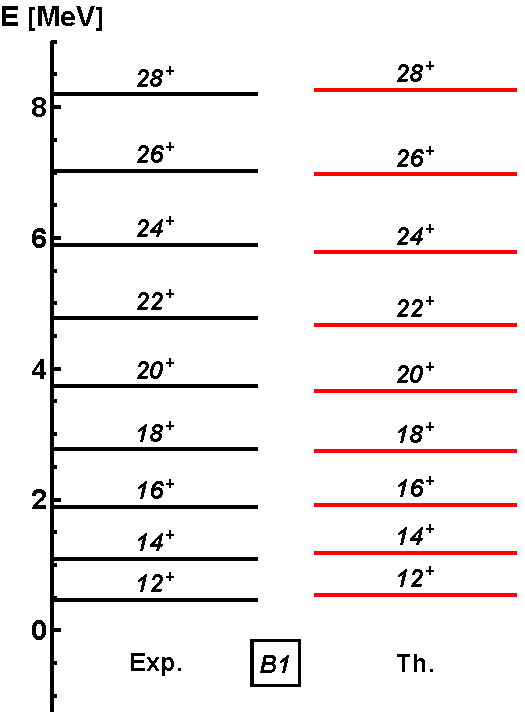
\includegraphics[width=0.46\textwidth]{Chapters/Figures/ba130-band1.pdf}
    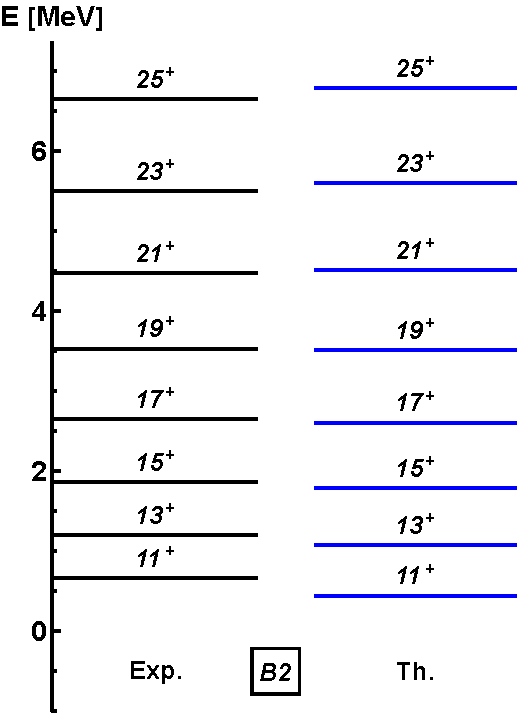
\includegraphics[width=0.46\textwidth]{Chapters/Figures/ba130-band2.pdf}
    \caption{Comparison between the experimental and theoretical excitation energies (Eq. \ref{excitation-energy-general-formula}) for the two wobbling bands of $^{130}$Ba (B1 and B2). Experimental data is taken from Ref. \cite{petrache2019diversity}. The theoretical data was obtained by fitting Eq. \ref{eq-wobbling-energy-evenA} as described in text, with the parameters defined in Table \ref{table-params-ba130}. Note that the band-head $I^\pi=10^+$ state from B1 is missing from the spectrum since it was subtracted from each level.}
    \label{plot-ba130-excitation-energies}
\end{figure}

Besides the excited spectrum obtained in Fig. \ref{plot-ba130-excitation-energies}, other quantities such as the rotational frequencies for the two bands in $^{130}$Ba are compared with experimental values in Fig. \ref{wobbling-energies-130ba-expVSth}, and the obtained results agree with the measured data quite well. Note that both frequencies are increasing functions of angular momentum, although for B1, at spin $I\geq 24\hbar$, there seems to be a less of an increase, which is not fully reproduced by the fitted values. Moreover, having the excitation energies for the two bands, one can evaluate the theoretical wobbling energies as defined in Eq. \ref{eq-wobbling-energy-definition-evenA} and compare them with the experimental values. The two quantities are graphically represented in Fig. \ref{wobbling-energies-130ba-expVSth}. Remarking the fact that there is an opposite behavior for the two curves, namely the experimental wobbling energies decrease with angular momentum, while the theoretical ones are constantly increasing. Unfortunately, it turns out that by using the Hamiltonian for a \emph{simple wobbler} is not enough to completely describe the collective motion in this isotope.

\begin{figure}
    \centering
    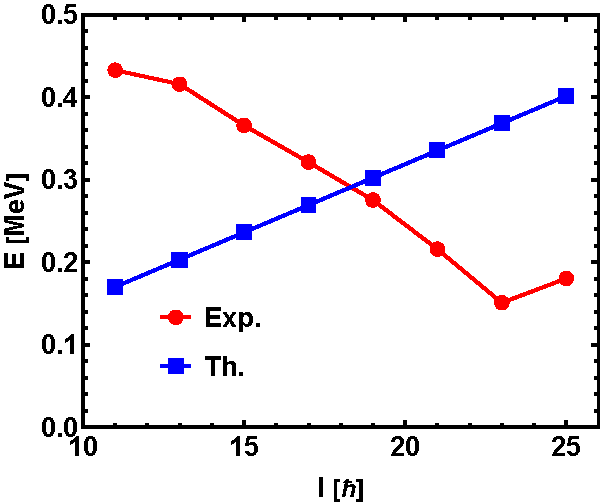
\includegraphics[scale=0.73]{Chapters/Figures/ba130-wobbling-energies.pdf}
    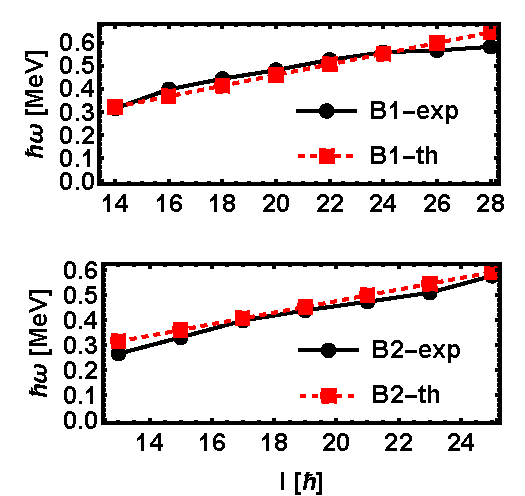
\includegraphics[scale=0.7]{Chapters/Figures/ba130-rotational-frequencies.pdf}
    \caption{\textbf{Left:} The wobbling energies for $^{130}$Ba calculated with Eq. \ref{eq-wobbling-energy-definition-evenA}. For the first state of B2, the energy was determined as $E_\text{wob}(11^+)=E_\text{B2}(11^+)-\frac{1}{2}E_\text{B1}(12^+)$ since the band-head state of B1 is zero (as per the definition of excitation energy given in Eq. \ref{excitation-energy-general-formula}). \textbf{Right:} The rotational frequencies for the two wobbling bands of $^{130}$Ba, calculated using Eq. \ref{rotational-frequency-canonical}.}
    \label{wobbling-energies-130ba-expVSth}
\end{figure}

\subsubsection*{Transition Probabilities}

Another step regarding the calculations for $^{130}$Ba consists of the electromagnetic transition probabilities. For this investigation some prior quantities are required. Firstly, the reduced transition probabilities $B(E2)$ (both the interband and the intraband) depend on the components $Q_{20}$ and $Q_{22}$ of the quadrupole moment. These two can be evaluated numerically using the expressions from Eq. \ref{quadrupole-components-q20-q22}, while the intrinsic quadrupole moment is furthermore evaluated using Eq. \ref{quadrupole-moment-Q0}. From the microscopic calculations performed by Chen et al. in Ref. \cite{chen2019transverse}, they determined that this isotope has a stable triaxial minimum located at $(\beta_2,\gamma)=(0.24,21.5^\circ)$. Within the following computations, this set of deformation parameters will be used. Taking the value of $\beta_2=0.24$, the intrinsic quadrupole moment $Q_0$ is readily obtained from Eq. \ref{quadrupole-moment-Q0}. The transition probabilities from Eqs. \ref{intraband-probability-simple-wobbler}, \ref{interband-probability-simple-wobbler-1}, and \ref{interband-probability-simple-wobbler-2} also depend on the two factors $w_{1,2}$ defined in Eq. \ref{eqs-w1-w2-terms-wobbling}, which are functions of the three moments of inertia. Thus, the quality of the fitting procedure will also reflect the calculus for the transition probabilities through $\mathcal{P}_\text{fit}$. The numerical values for $Q_0$, $w_{1,2}$, and $Q_{20,22}$ are presented in Table \ref{transition-parameters-ba130}. Having the deformation parameters, the $w_{1,2}$ terms, and the quadrupole components, one can evaluate the reduced transition probabilities. 

\begin{table}
    \centering
    \begin{tabular}{|c|c|c|}
    % \begin{tabular}{|p{0.15\linewidth}|p{0.25\linewidth}|p{0.5\linewidth}|}
    \hline
    Parameters & Calculated values & Observations                                               \\ \hline
    $\beta_2$  & 0.24              & Taken from Ref. \cite{chen2019transverse}                 \\ \hline
    $\gamma$   & $21.4^\circ$      & Taken from Ref. \cite{chen2019transverse}                 \\ \hline
    $w_1$      & 1.008             & Evaluated with $\mathcal{P}_\text{fit}$                    \\ \hline
    $w_2$      & 0.132             & Evaluated with $\mathcal{P}_\text{fit}$                    \\ \hline
    $Q_0$      & 390.376 $eb\cdot10^{-2}$      & As per Eq. \ref{quadrupole-moment-Q0}                                                           \\ \hline
    $Q_{20}$   & 363.213 $eb\cdot10^{-2}$          & As per Eq. \ref{quadrupole-components-q20-q22}                                                            \\ \hline
    $Q_{22}$   & 101.168 $eb\cdot10^{-2}$           & As per Eq. \ref{quadrupole-components-q20-q22}                                                            \\ \hline
    $B(E2)_\text{in}$ &        0.0509047 $(eb)^2$          & Eq. \ref{intraband-probability-simple-wobbler}              \\ \hline
    \end{tabular}%
    \caption{The numerical values for the quantities which are required to determine the quadrupole transition probabilities $B(E2)$ defined in Eqs. \ref{intraband-probability-simple-wobbler} - \ref{interband-probability-simple-wobbler-2}. The parameter set $\mathcal{P}_\text{fit}$ was obtained through the fitting procedure and the values are shown in Table \ref{table-params-ba130}. The intraband transition probabilities $B(E2)$ are evaluated for states $(n,I)\to(,,I-2)$.}
    \label{transition-parameters-ba130}
\end{table}

The graphical representation from Fig. \ref{BE2out-transitions-130ba} shows the interband transition probabilities $B(E2)_\text{out}$ for states $(n_w=1,I)\to(n_w=0,I-1)$. These values are determined with the parameters defined in Table \ref{transition-parameters-ba130}. A constant decrease with spin can be observed, and an overall agreement with theoretical calculations from Ref. \cite{chen2019transverse} is observed (see inset $a$ from Fig. 4).

\begin{figure}
    \centering
    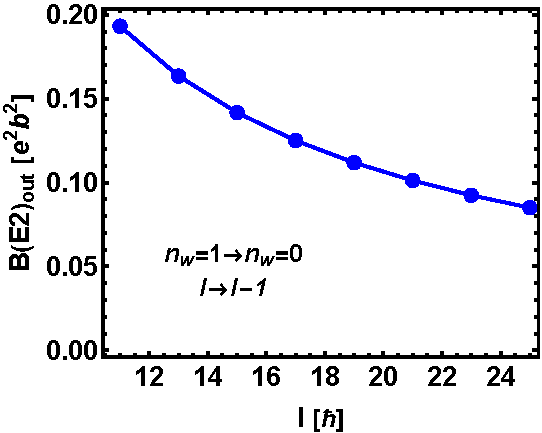
\includegraphics[scale=0.65]{Chapters/Figures/BE2-out-130Ba.pdf}
    \caption{The interband quadrupole transition probabilities (Eq. \ref{interband-probability-simple-wobbler-1}) from the first excited wobbling band (B2) to the yrast band (B1) for $^{130}$Ba.}
    \label{BE2out-transitions-130ba}
\end{figure}

\subsubsection*{Harmonic Approximation - General Discussion}

Even though the spectrum of this even-even nucleus has been quantitatively reproduced quite well and the values for the tree obtained MOI indicate a triaxial nucleus with main rotation around the third axis, it should not be considered a `realistic' tool in describing this isotope. This is because in another work, Chen et al. \cite{chen2019transverse} found through microscopic calculations that the wobbling motion does not occur as per a pure triaxial rotator, but it emerges from the coupling of two quasi-particles $\pi(h_{11/2})^2$ with a triaxial core. In fact, their work shows that $^{130}$Ba is the first nucleus in which a configuration with two quasi-particles generates stable triaxial deformation through wobbling motion. Consequently, the numerical implementation performed here only shows that HA can be a suitable tool to show that $^{130}$Ba does behave as a wobbler, but this pure triaxial rotator model \emph{hides} contributions coming from single-particle configuration within the final Hamiltonian. This translates to the fact that Eq. \ref{eq-wobbling-energy-evenA} contains the effect of the two $h_{11/2}$ protons hidden within $\hbar\omega_w$. In fact, looking back at $E_\text{wob}$ from Fig. \ref{wobbling-energies-130ba-expVSth}, the discrepancy of the two lines is a clear indicator that some other terms should be taken into account. Nevertheless, this simple and straightforward formalism used to describe the wobbling bands in the even-even $^{130}$Ba nucleus proves to be a decent tool. The calculations presented here have been done independently by the current team, and the obtained results are unique to this present research.

Concluding this section on wobbling motion of even-even nuclei, a final sketch is depicted in Fig. \ref{simple-wobbler-geometrical-schematic}, where the main axes of the triaxial ellipsoid are represented and denoted with $m$, $s$, and $l$-axis (medium, short and long, respectively). The precession motion of the total angular momentum (the a.m. of the core itself) will be around the $m$-axis, having the largest moment of inertia.

\begin{figure}
    \centering
    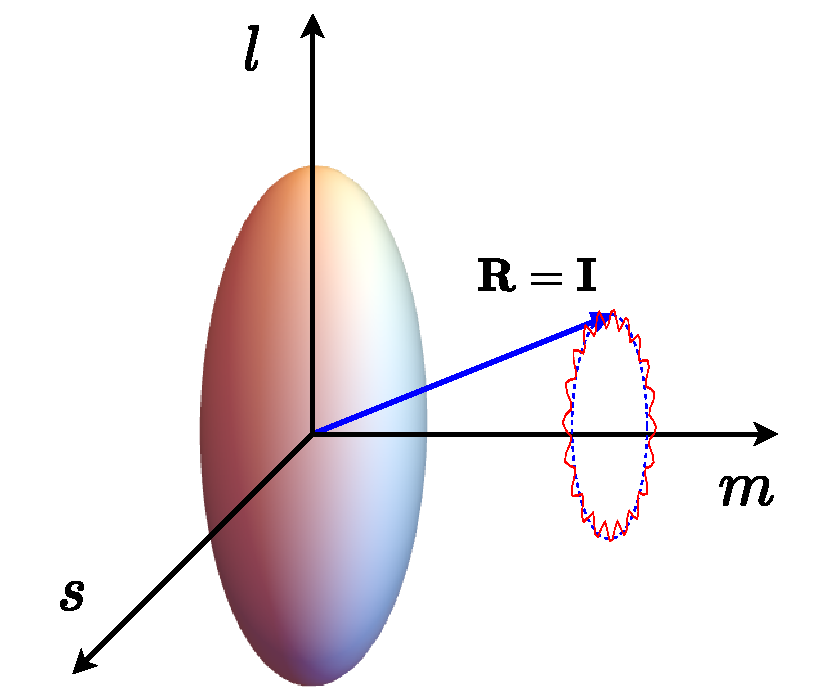
\includegraphics[scale=0.65]{Chapters/Figures/simple-wobbler.pdf}
    \caption{A schematic representation with a \emph{simple wobbler}, with the total angular momentum doing a precessional motion about the axis with largest MOI. In this particular sketch, the axis with largest MOI is denoted with $m$ for intermediate/medium. $l$- and $s$-axis represent the long and short axes, respectively. The small-amplitude oscillations of $\mathbf{R}$ are depicted with the (red) encircled sine wave. This figure was adapted from Ref. \cite{poenaru2021extensive} and inspired from Ref. \cite{sensharma2020longitudinal}.}
    \label{simple-wobbler-geometrical-schematic}
\end{figure}

\section{Wobbling Motion in Odd-Mass Nuclei}